\subsection{Projektumweltanalyse}

Die Projektumweltanalyse visualisiert interne und externe Beziehungen zu einem Projekt. Sie dient der Identifikation von Einflussfaktoren auf das Projekt (sowohl positive als auch negative). Anhand der Projektumweltanalyse können die Projektmitglieder die Auswirkungen der Einflussfaktoren auf das Projekt abschätzen und entsprechende Maßnahmen ergreifen. \citev{projektumweltanalyse}

\begin{figure}[H]
    \centering
    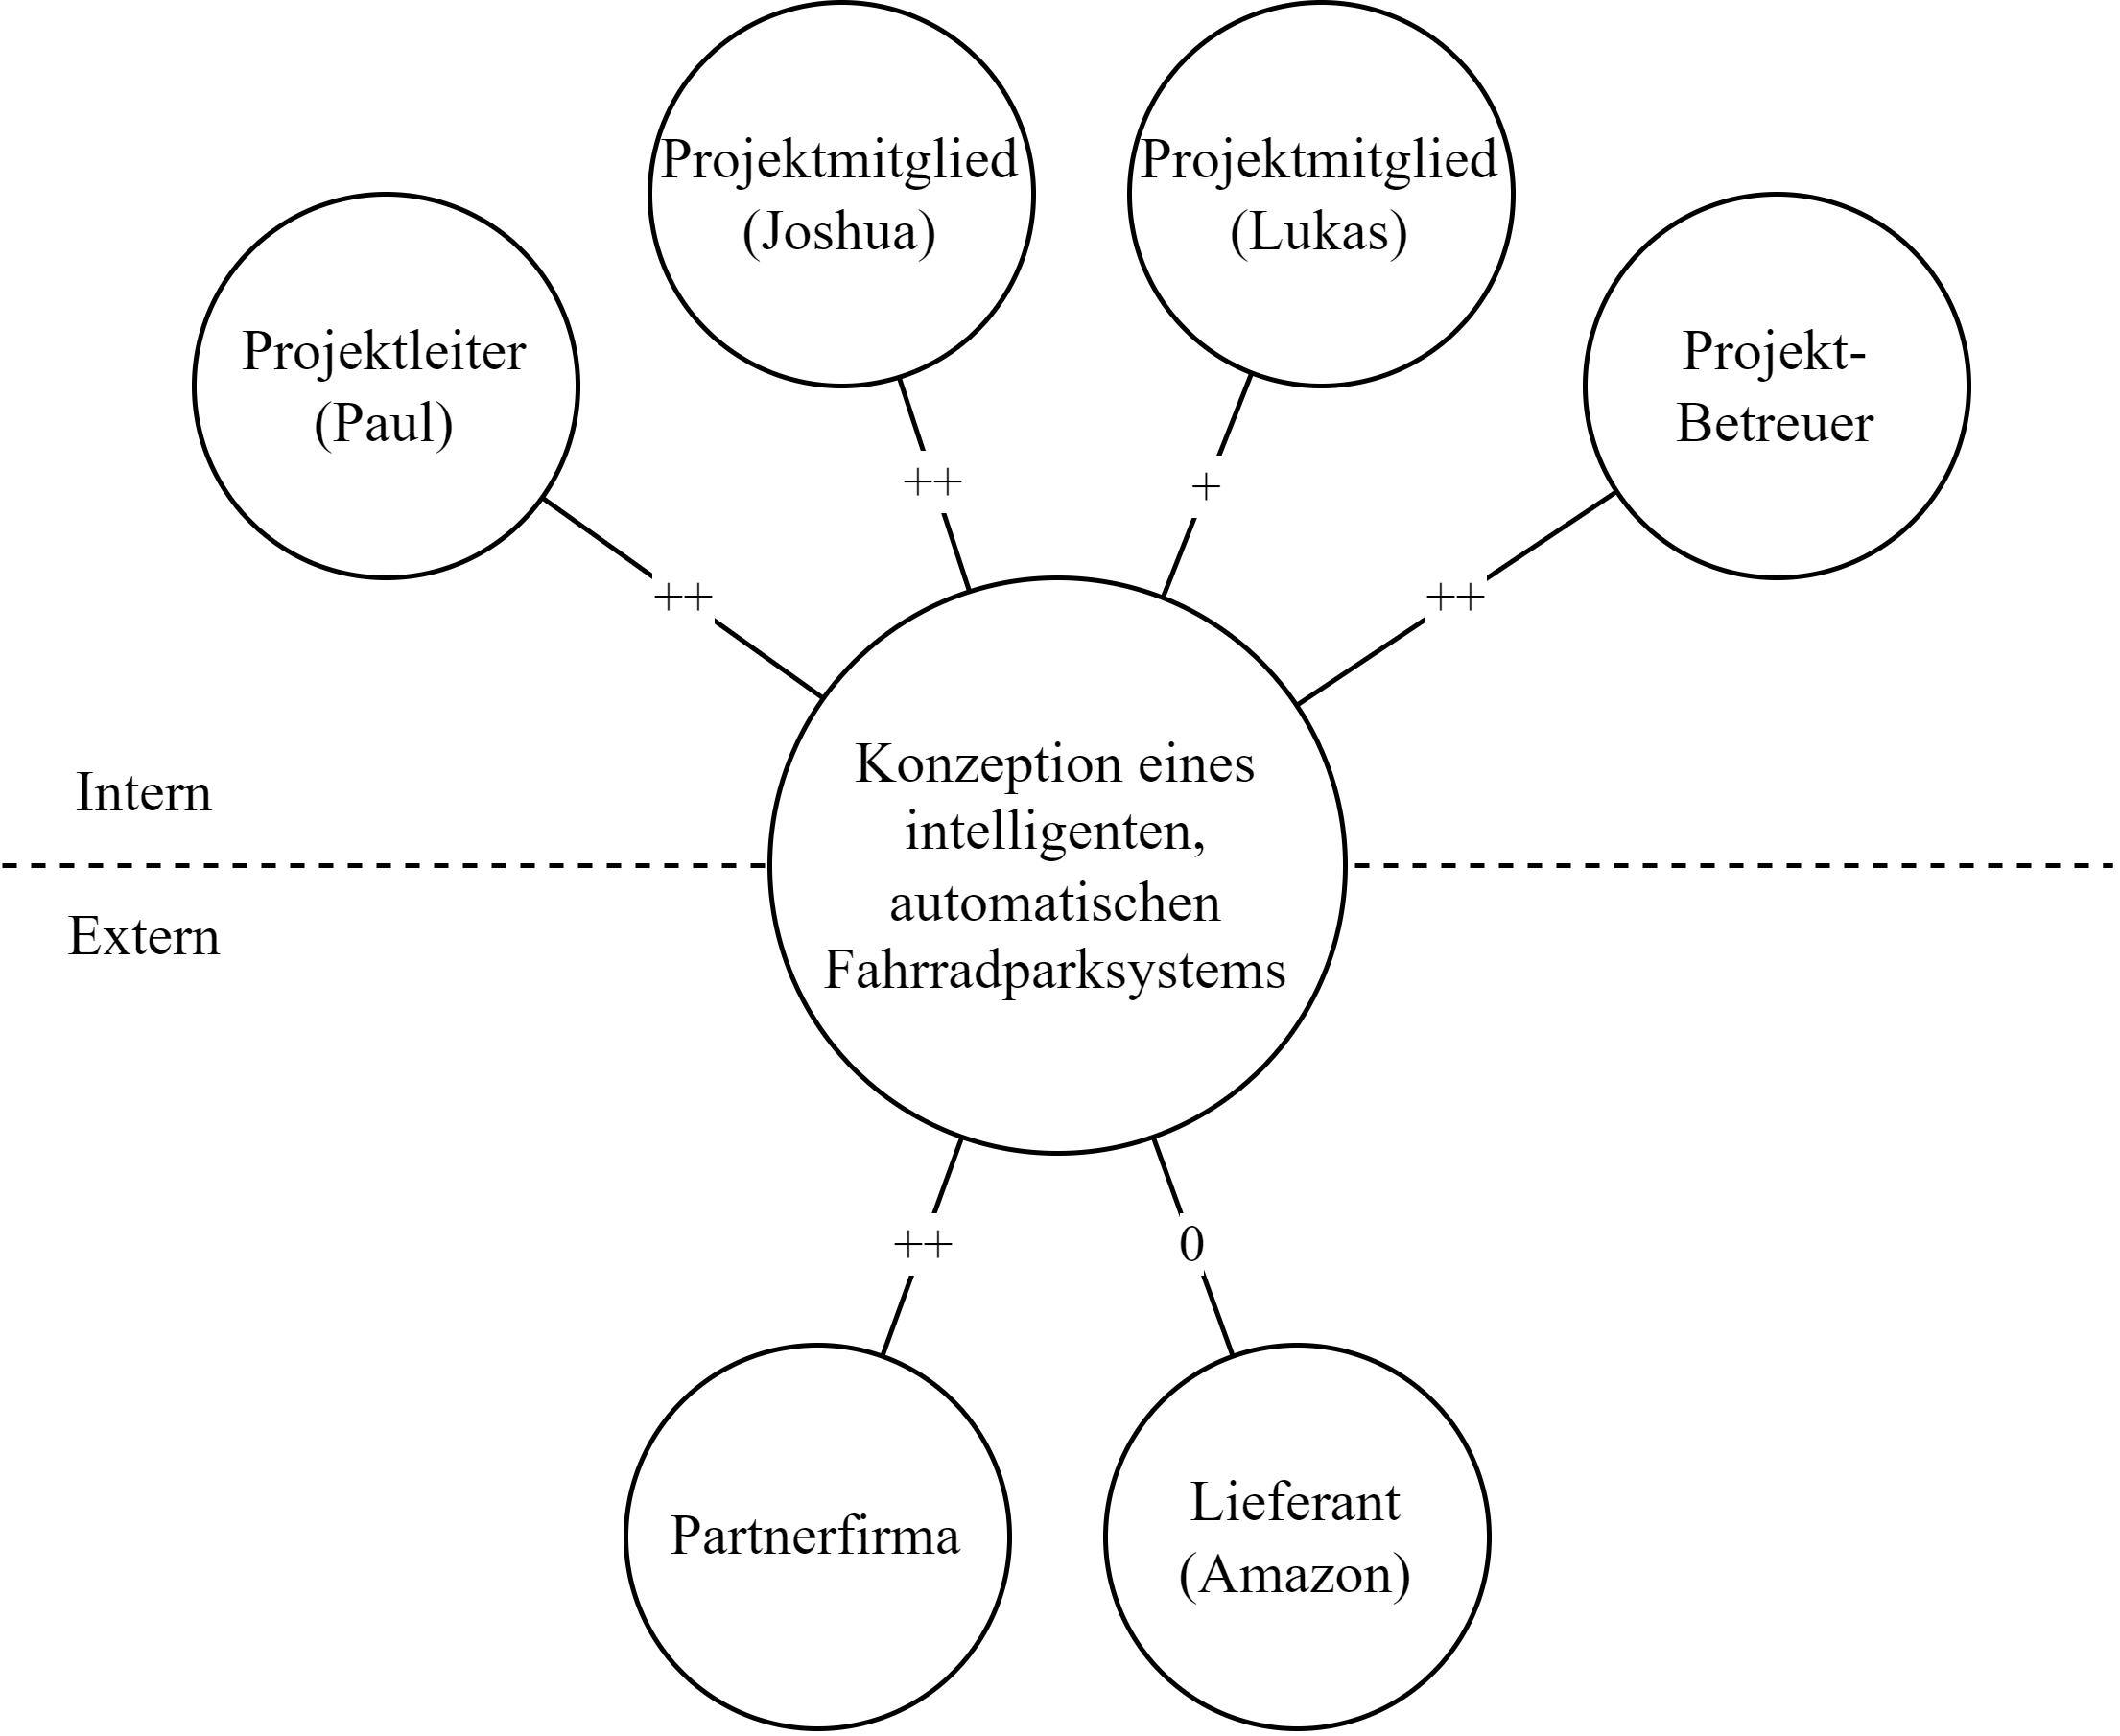
\includegraphics[width=0.8\textwidth]{images/projektumweltanalyse.png}
    \caption{Projektumweltanalyse}
    \label{fig:projektumweltanalyse}
\end{figure}